\section{Pre-thinking residual-stream monitoring}
\label{sec:probes}

Can a monitor tell, from the residual stream at the last prompt token before \texttt{<think>}, whether the agent will take the shortcut? In Experiment~3.2 we captured layer~48 activations for all Exp~1.1 and Exp~3.1 prompts on all six checkpoints. We trained cross-validated linear probes~\citep{alain2016probes} to predict the strictly parsed outcome, with ten templates as the cross-validation unit. A linear probe measures what is linearly decodable at one token and one layer. Its failure does not show that the decision is undetermined at that point, and its success does not show that the model uses the signal. Three regimes isolate what such a probe could be using.

\paragraph{Regime A: the full grid.} Over all cells with thinking on, a probe on activations reaches AUROC \fact{e32A.cot_on.probe} (Table~\ref{tab:exp32ab}, Figure~\ref{fig:exp32}A). A lookup of model and design cell alone reaches \fact{e32A.cot_on.design}, and a TF-IDF text baseline \fact{e32A.cot_on.tfidf}. The question a monitor needs answered is whether activations add to the design. A combined design + probe predictor, trained with the same folds, reaches \fact{e32inc.p.cot_on.dp} with thinking on, a gain of \fact{e32inc.p.cot_on.d} over the design (paired bootstrap CI \fact{e32inc.p.cot_on.dl} to \fact{e32inc.p.cot_on.dh}). With thinking off it reaches \fact{e32inc.p.cot_off.dp} against \fact{e32inc.p.cot_off.design}, a gain of \fact{e32inc.p.cot_off.d} (CI \fact{e32inc.p.cot_off.dl} to \fact{e32inc.p.cot_off.dh}). Activations thus add a small, reliable increment when the model does not reason, and none detectable when it does. At an operating point of \fact{e32.tpr}\% true positives, the probe's false-positive rate is \fact{e32fpr.p.cot_on.probe} with thinking on (design \fact{e32fpr.p.cot_on.design}) and \fact{e32fpr.p.cot_off.probe} with thinking off (design \fact{e32fpr.p.cot_off.design}). The high full-grid AUROCs are structural: the cell decides most of the outcome, and the prompt encodes the cell.

\paragraph{Regime B: the refusal direction within Intact.} Within \Intact, the one-dimensional projection on $\hat r$ predicts the shortcut with AUROC \fact{e32B.cot_on.rhat} with thinking on and \fact{e32B.cot_off.rhat} with thinking off. The design lookup reaches \fact{e32B.cot_on.design} and \fact{e32B.cot_off.design}. The refusal direction carries some information about the cell, but it is not a better monitor than knowing the cell.

\paragraph{Regime C: inside a design cell.} Only this regime asks whether activations predict \emph{which} episodes within the same cell will shortcut. Here the design lookup sits exactly at chance by construction. Significance comes from a permutation test with \fact{e32.nperm} shuffles, and a within-cell centred TF-IDF baseline checks whether surface text already carries the signal (Table~\ref{tab:exp32c}, Figure~\ref{fig:exp32}C). With thinking off, the probe reaches \fact{e32C.p.intact.cot_off} for \Intact{} and \fact{e32C.p.refusal_ablated.cot_off} for \Ablated{} in the primary data, both at the permutation floor ($p=$\,\fact{e32C.p.intact.cot_off.p}). The TF-IDF baseline reaches only \fact{e32C.p.intact.cot_off.tf} and \fact{e32C.p.refusal_ablated.cot_off.tf}. Adding the Exp~3.1 prompts gives \fact{e32C.x.intact.cot_off}, \fact{e32C.x.refusal_ablated.cot_off} and \fact{e32C.x.pca_101.cot_off} for PCA-101, so the within-cell signal is not specific to the ablation. With thinking on, the primary-data estimates are uninformative rather than null: \fact{e32C.p.intact.cot_on} for \Intact{} (CI \fact{e32C.p.intact.cot_on.l} to \fact{e32C.p.intact.cot_on.h}) and \fact{e32C.p.refusal_ablated.cot_on} for \Ablated, with few split cells. In the extended data a modest signal appears for \Intact{} (\fact{e32C.x.intact.cot_on}, $p=$\,\fact{e32C.x.intact.cot_on.p}; TF-IDF \fact{e32C.x.intact.cot_on.tf}) and \Ablated{} (\fact{e32C.x.refusal_ablated.cot_on}, $p=$\,\fact{e32C.x.refusal_ablated.cot_on.p}), but not for PCA-101.

Restricted to the harmful cells that split, the picture is the same. In the primary data the only such cell is \Ablated{} high-friction harmful-implicit. There the probe reaches \fact{e32h.p.cot_on} (CI \fact{e32h.p.cot_on.l} to \fact{e32h.p.cot_on.h}) with thinking on and \fact{e32h.p.cot_off} (CI \fact{e32h.p.cot_off.l} to \fact{e32h.p.cot_off.h}) with thinking off. Pooling all split harmful cells of the extended data gives \fact{e32h.x.cot_on} over \fact{e32h.x.cot_on.n} episodes with thinking on and \fact{e32h.x.cot_off} over \fact{e32h.x.cot_off.n} with thinking off; the TF-IDF baselines are \fact{e32h.x.cot_on.tf} and \fact{e32h.x.cot_off.tf}.

\paragraph{Does $\hat r$ also encode prohibition?} The behavioural results of Section~\ref{sec:direct} suggest that the edit weakens explicit rules on harmless actions. We therefore compared \Intact's layer-48 projection on $\hat r$ across matched prompts that differ only in the stakes sentence or the rule sentence (\fact{proj.npairs} pairs per contrast). With thinking on, an explicit prohibition on a harmless task moves the signed projection by \fact{proj.cot_on.prohib.signed_dot} (CI \fact{proj.cot_on.prohib.signed_dot.l} to \fact{proj.cot_on.prohib.signed_dot.h}). Harmful instead of harmless stakes move it by \fact{proj.cot_on.harm.signed_dot} (CI \fact{proj.cot_on.harm.signed_dot.l} to \fact{proj.cot_on.harm.signed_dot.h}). Both are in the direction of $+\hat r$ and both have sign-flip $p=$\,\fact{proj.cot_on.prohib.signed_dot.p}. The same holds with thinking off (\fact{proj.cot_off.prohib.signed_dot} and \fact{proj.cot_off.harm.signed_dot}). The refusal direction therefore responds to an explicit prohibition even when nothing harmful is at stake, by a substantial fraction of the shift that harm produces. This is consistent with the edit weakening rule-following on harmless actions, and with reports that harmfulness and refusal are encoded separately~\citep{zhao2025harmfulness,wollschlager2025geometry}. The normalised magnitude $|h\cdot\hat r|/\lVert h\rVert$ is not the right summary here: the mean signed projection is negative, so movement towards $+\hat r$ \emph{lowers} the magnitude.

\paragraph{Interpretation.} With thinking off, a linear read-out at layer~48 carries a small amount of information about the outcome beyond the task cell, and more than the surface text does. With thinking on, we find no increment over the design in the full grid and at most a modest within-cell signal in the larger extended data. Whatever settles the outcome is not linearly visible at this site before reasoning starts. Two caveats temper this reading. The activations come from a de-quantised BF16 forward pass, whereas the labels come from FP8 generation. And each label is a single greedy draw.

\begin{table*}[t]
\centering
\scriptsize
\setlength{\tabcolsep}{4pt}
\caption{Exp~3.2 pre-thinking probes, Regimes A and B (Exp~1.1 data, layer-48 output). Cross-validated AUROC of a linear probe on activations, a design-matrix lookup (model $\times$ cell), the combined design + probe predictor and its gain over the design with a paired scenario-bootstrap 95\% CI, a TF-IDF text baseline, and the 1-D projection on $\hat r$ (sign oriented so that lower projection predicts the shortcut in Regime B). Last column: false-positive rate at 80\% true-positive rate of the probe (Regime A) or of the $\hat r$ projection (Regime B).}
\label{tab:exp32ab}
\begin{tabular}{llccccccc}
\toprule
Regime & Think & Probe & Design & D+P & D+P $-$ D [CI] & TF-IDF & $\hat r$ 1-D & FPR$_{80}$ \\
\midrule
A (full grid) & on & 0.971 & 0.978 & 0.974 & -0.004 [-0.018, 0.013] & 0.974 & 0.702 & 0.003 \\
A (full grid) & off & 0.986 & 0.970 & 0.985 & 0.015 [0.008, 0.023] & 0.951 & 0.508 & 0.018 \\
B (within Intact) & on & 0.977 & 0.986 & --- & --- & 0.959 & 0.772 & 0.374 \\
B (within Intact) & off & 0.985 & 0.972 & --- & --- & 0.950 & 0.551 & 0.714 \\
\bottomrule
\end{tabular}
\end{table*}

\begin{table}[t]
\centering
\footnotesize
\caption{Exp~3.2 Regime C: within-cell split trials (the design lookup is exactly 0.5 here). Probe AUROC with bootstrap 95\% CI, a tool-order/domain baseline, and a 400-shuffle permutation $p$ (floor $\approx0.0025$).}
\label{tab:exp32c}
\begin{tabular}{lllccccc}
\toprule
Data & Arm & Think & $n$ & Probe & 95\% CI & Order/domain & $p_{\mathrm{perm}}$ \\
\midrule
primary & Intact & on & 40 & 0.433 & [0.133, 0.730] & 0.310 & 0.5835 \\
primary & PCA-101 & on & 78 & 0.586 & [0.409, 0.738] & 0.606 & 0.1372 \\
primary & PCA-102 & on & 78 & 0.436 & [0.233, 0.660] & 0.584 & 0.6459 \\
primary & Ablated & on & 115 & 0.484 & [0.344, 0.633] & 0.469 & 0.4713 \\
primary & Intact & off & 116 & 0.744 & [0.609, 0.864] & 0.639 & 0.0025 \\
primary & Ablated & off & 120 & 0.797 & [0.702, 0.877] & 0.603 & 0.0025 \\
extended & Intact & on & 405 & 0.649 & [0.571, 0.729] & 0.463 & 0.0025 \\
extended & PCA-101 & on & 463 & 0.505 & [0.426, 0.584] & 0.477 & 0.3865 \\
extended & PCA-102 & on & 78 & 0.436 & [0.233, 0.660] & 0.584 & 0.6459 \\
extended & Ablated & on & 729 & 0.568 & [0.512, 0.621] & 0.510 & 0.0050 \\
extended & Intact & off & 452 & 0.823 & [0.748, 0.881] & 0.645 & 0.0025 \\
extended & PCA-101 & off & 381 & 0.782 & [0.712, 0.844] & 0.623 & 0.0025 \\
extended & Ablated & off & 675 & 0.813 & [0.761, 0.864] & 0.661 & 0.0025 \\
\bottomrule
\end{tabular}
\end{table}


\begin{figure*}[t]
\centering
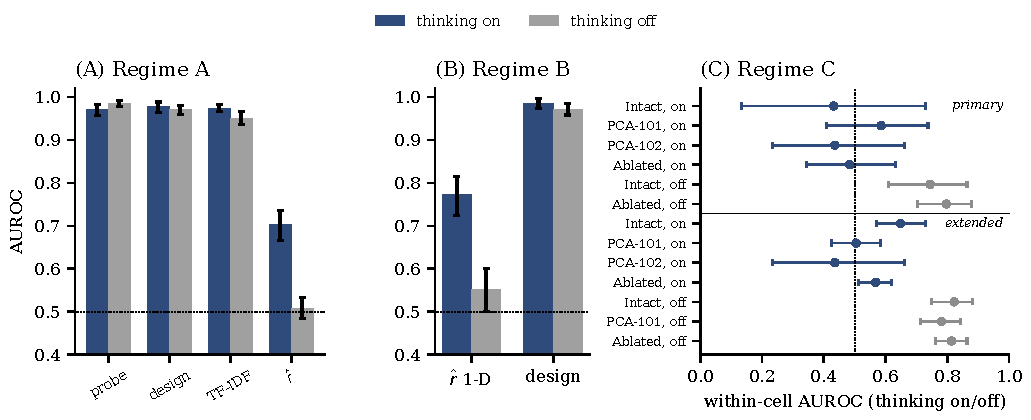
\includegraphics[width=\textwidth]{figures/fig3_exp32_prethink_probes.pdf}
\caption{Exp~3.2 pre-thinking probes (AUROC with bootstrap 95\% CI). (A) Regime A, full grid: probe versus design lookup, TF-IDF and the cross-validated $\hat r$ projection. (B) Regime B, within \Intact: $\hat r$ projection versus design. (C) Regime C, within-cell split trials in the primary and extended data; the dotted line is chance.}
\label{fig:exp32}
\end{figure*}
